\documentclass[titlepage]{article}
\usepackage{amssymb,amsthm}
\usepackage{amsfonts,amsmath}
\usepackage{color}
\usepackage{graphicx}
\usepackage{epstopdf}
\usepackage{dashrule}
\usepackage[margin = 1in]{geometry}
\geometry{
  lmargin=1.5in
}
\usepackage{fancyhdr}
\pagestyle{fancy}
\fancyhf{}
\renewcommand{\headrulewidth}{0pt}
\usepackage{setspace}
\usepackage{listings}
% \doublespacing
\def\vnew{v_{new}}
\def\iso{\cong}
\def\moneq{\equiv}
\newtheorem{theorem}{Theorem}
\theoremstyle{definition}
\newtheorem{claim}{Claim}
\newtheorem{conjecture}{Conjecture}
\theoremstyle{proof}
\def\neg{^{-1}}
\def\N{\mathbb N}
\def\W{\mathcal W}
\def\A{\mathcal A}
\ifx \ser \undefined
\newcommand \ser[2][i]{\{#2_{#1}\}_{#1=1}^\infty}
% use like
% $\ser{W}$
% $\ser[j]{N}$
\fi

\ifx \addtotoc \undefined
\newcommand \addtotoc[2][]{\addcontentsline{toc}{section}{\numberline{#1}#2}}
\fi


\begin{document}

% the math paper I found had
% permission
% title
% ii approved
% iii contents
% iv list of figures
% v abstract
% 1 start of paper...
% 24 references

% going by arrangement rather than the example
%1 permission to copy page


\begin{minipage}[h]{5in}
  I give permission for public access to my Honors paper
  and for any copying or digitization to be done
  at the discretion of the College Archivist and/or the College Librarian.

  \vspace{1in}
  Signed \hrulefill

  \vspace{.5in}
  Preston Tunnell Wilson \hdashrule{3.58in}{1pt}{1pt}

  \vspace{.5in}
  Date \hrulefill
\end{minipage}

\newpage

% 2 title page
\rhead{\thepage}
\pagenumbering{roman}
\title{
  Comparing Various Locomotion Methods within Virtual Environments
}

\author{
  Preston Tunnell Wilson }

\date{
  Department of Mathematics and Computer Science\\
  Rhodes College\\
  Memphis, Tennessee\\
  \vspace{2in}
  2016\\
  \vspace{2in}
  Submitted in partial fulfillment of the requirements
  for the Bachelor of Science degree with Honors in Computer Science
}

\maketitle

% 3 signature page
\setcounter{page}{2}
\noindent This Honors paper by
\underline{Preston Tunnell Wilson \hfill}

\noindent has been read and approved for Honors in\\
\underline{the Department of Mathematics and Computer Science}.

\begin{center}
  \begin{minipage}[h]{3in}
    \centering
    \vspace{1in}
    \hrulefill\\
    Dr. Betsy Sanders\\
    Project Advisor 

    \vspace{1in}
    \hrulefill\\
    Dr. Mike Sheard\\
    Second Reader

    \vspace{1in}
    \hrulefill\\
    Dr. Jamie Jirout\\
    Extra-Departmental Reader

    \vspace{1in}
    \hrulefill\\
    Dr. Mike Sheard\\
    Department Chair
  \end{minipage}
\end{center}
% include signatures
\newpage
% 4 acknowledgement page

% all sections folowing the content page are included in the Contents
\tableofcontents

\newpage
\addtotoc{List of Figures}
\listoffigures

% this needs to be numbered too
% no longer than 250 words and double spaced
% currently 232
\begin{abstract}
  \thispagestyle{fancy}
  \setcounter{page}{5}
  \addtotoc{Abstract}
  \doublespacing
  Two inexpensive methods of exploring a virtual environment are walking in place (WIP) and arm swinging.
  These techniques are compelling because
  they strike a balance between space requirements, cost, and proprioceptive cues.
  They seem to provide better spatial awareness of a virtual environment
  than other inexpensive virtual navigation techniques such as joysticks or controllers.
  On the other hand, they are much cheaper and require less space than tracking systems.
  In our prior work, we had success in implementing a WIP method
  using an inexpensive Nintendo Wii Balance Board.
  We showed that participants' spatial orientation was the same as normal walking
  and superior to joystick navigation.

  We seek to extend our previous work utilizing the Myo armband--
  an inexpensive wearable device (199 USD)
  with electromyography sensors, gyroscopes, and accelerometers.
  We previously found that our arm swinging method outperforms a simple joystick
  and that spatial orientation is comparable to physically walking on foot.

  In this work, we compare physical locomotion to both arm swinging and WIP.
  We implement these methods with Myo armbands.
  Both algorithms let users freely explore an HMD-based virtual environment.
  We tested users' spatial orientation and distance estimation.
  Interestingly, our mean turning angle errors were higher than those in our previous studies.
  Also notable is that users performed better at blind walking in the WIP condition than in physical locomotion.
\end{abstract}

% each chapter on a new page
\doublespacing
\pagenumbering{arabic}

% from thingy
\section{Introduction}
Immersive virtual environments (IVEs) allow people to learn about
an environment which for reasons of time, distance, expense, and
safety would not otherwise be available.
Virtual systems that result in high-fidelity interactions can be important tools for learning and training.
A virtual flight simulator is an example of a virtual system that provides a strong connection between real action
and virtual experience and is commonly used to train pilots \cite{trove.nla.gov.au/work/12170008}.
IVEs have also been used to safely train miners \cite{vanWyk2009VRT15034541503465},
assess the evacuation plans of a building before it is built \cite{Ruppel2011DBS2043741.2043863},
educate doctors and nurses \cite{torkington},
provide therapy for post-traumatic stress disorder \cite{rothbaum},
teach children about many different topics such as planetary phenomena \cite{doi:10.1080/09500690305027},
help treat kids with autism \cite{mitchell},
and so on.
Moreover, with the recent release of commodity level head-mounted displays (HMDs) like the Oculus Rift (350 USD),
virtual reality systems could have a broader impact on
education, entertainment, medicine, architecture, and training.
However, they are not widely used because of their delicacy and complexity.
With the recent invention of inexpensive devices like the Microsoft Kinect,
Thalmic Labs Myo armband, and Nintendo Wii components,
creation of a high-fidelity, low-cost virtual reality system might become a reality.
We now have the opportunity to make IVEs pervasive in a way that we have not seen before.

Since inexpensive haptic devices like joysticks have been shown to cause
disorientation in IVEs \cite{Chance1998:Presence,Ruddle2006:FENS,Lathrop2002:PO},
it is not clear how to effectively and inexpensively explore an IVE.
Finding ways to spatially navigate in IVEs that perform comparably to the way we navigate in the
real world is a challenging and important problem that has received significant attention.
In the real world, humans naturally spatially
update their location with respect to objects in their environment.
This phenomenon can happen in an IVE, but there are some limitations \cite{kelly}.
A significant body of work has shown that
physical movement aids in spatial orientation \cite{Ruddle2006:FENS,waller}.
That is, exploring an IVE by physically walking results in the most realistic experience.
Moreover, a user's spatial orientation in an IVE is best when the proprioceptive
cues of walking match the visual input \cite{Ruddle:2009:BUW:1502800.1502805}.
Physically walking in an IVE requires that the physical location of the user be obtained from
some sort of tracking device.
Moreover, tracking systems are expensive, limit exploration to the size of the tracking system, and
the physical space requirements suggest that it will never be a commodity level product.

We turn our attention to alternatives which avoid these constraints.
Two inexpensive methods of exploring a virtual environment are ``walking in place'' (WIP) and arm swinging.
These techniques are compelling because they seem to provide more proprioceptive cues
than traditional inexpensive virtual navigation techniques like a joystick.
More specifically, WIP and arm swinging seem to result in better spatial awareness of the environment.
For example, in our prior work,
we had success in implementing a WIP method
using an inexpensive Nintendo Wii Balance Board \cite{Williams:2011:EWP}.
We showed that participants' spatial orientation was the same as normal walking and superior to joystick navigation \cite{Williams:2011:EWP}.

We implemented an alternative WIP algorithm later with Microsoft Kinect sensors \cite{Wilson:2014}.
However, we found some problems using it as the basis of a virtual environment system.
The most immediate trouble was occlusion of body parts:
when the user was facing certain orientations,
the Kinect would not be able to correctly determine the user's skeletal data.
We tried to remedy this by adding an additional Kinect to our system,
but this did not completely solve the problem.
To prevent the faulty Kinect data from causing users to shift forward unintentionally,
we increased the angle of the inner knee necessary to record a step.
This forced the users to practically march rather than walk in place.
Users found this to be uncomfortable.
Finally, users could only move forward in full step increments--
users did not have precise control over their movement.

Recently, we used a Myo armband (199 USD)
to implement a simple arm swinging algorithm that allowed a user to freely explore an HMD-based virtual environment \cite{previousMYO}.
We found that our arm swinging method outperforms a simple joystick and that spatial orientation is comparable to physically walking on foot \cite{previousMYO}.
Both walking in place and arm swinging locomotion methods do not suffer from the same space constraint as tracking systems do.


The purpose of this paper is to present and analyze our comparison of various navigation methods.
We primarily make use of the Myo armband.
The Myo armband is a wearable device with various sensors as seen in Figure \ref{fig:morgan}.
We describe a walking in place algorithm that is implemented using a Myo worn around the middle part of the calf.
We believe that this method of implementing walking in place is more robust and simpler to implement than our previous algorithms \cite{Williams:2011:EWP,Wilson:2014}.
We compare this algorithm to our previous arm swinging algorithm as well as physically walking.
This comparison is done with spatial orientation tasks,
blind walking tasks, and user surveys.
We conducted this study on 12 participants in a within-subjects design.

The within-subject experiment presented in this work compares
subjects' spatial orientation and distance perception under three different locomotion conditions:
Myo walking in place, Myo arm swinging, and physically walking.
In all three methods, subjects rotate physically.
In both the Myo arm swinging and the Myo walking in place conditions, subjects translate in
the yaw direction that they are looking.
Spatial orientation is used
to evaluate navigation because learning the layout and the information in the environment is often the goal of a virtual system.
For example, a student walking home from school must identify his or
her location and direction within the surrounding environment before determining in which direction to proceed.
This sense of spatial orientation relies heavily on visual information and whole-body
information while moving in an environment \cite{wartenberg:book}.
In other words, both environmental cues and path integration (the process of integrating self-motion cues over time) inform
spatial orientation.
Thus, spatial orientation is generally tested by
performing experiments that require participants to combine the use
of environmental cues and path integration.
A popular way to assess a user's spatial orientation in an IVE
is to measure turning errors and latencies in tasks where subjects are asked to turn to face
previously learned target objects \cite{may} .
To measure spatial
orientation, we recorded the turning errors and latencies associated
with subjects turning to face a remembered object from different
positions in the IVE.
Turning error is defined as the difference between the subjects' actual facing direction and direction needed to
face the target correctly.

\newpage
\section{Locomotion Implementation}
Our three locomotion methods,
walking in place, arm swinging, and physical tracking,
required the following pieces of technology:
\begin{itemize}
\item Two Myo armbands (199 USD each)
\item WorldViz Precision Point Tracking System (40,000 USD)
\item Vizard Virtual Reality Software (870 USD)
\item Unity 3d Game Engine (Free)
\item Oculus Rift Developers Kit 2 (350 USD)
\end{itemize}

Due to technical difficulties,
the Oculus Rift would not display the Vizard virtual environment
which we had used previously.
Thus, we switched to Unity.
This gave us an opportunity to re-implement our code.
Over five years, our experiment code accrued a lot of cruft and a lot of state-dependent logic.
In this re-write, we focused on modularizing our code
and making what parts we could functional rather than state-dependent.

We divided the logic as follows:
\begin{itemize}
\item Experiment code:
  this code started the experiment,
  directed the user through the experiment,
  and wrote the results to a file.
  It was dependent on:
  \begin{itemize}
  \item Object controller:
    this code managed the objects which users turned to face.
    It would switch out the objects when the user progressed between trials,
    and would return to the experiment code the objects which the user should turn to face.
    To account for effects of order, the locations subjects would visit and the objects they would face there
    were randomly ordered.
  \end{itemize}
\item Camera holder:
  Due to the way that Unity handles head mounted displays,
  we had to make a parent object to the camera.
  Thus, the camera object could \emph{rotate} freely
  while it inherited the \emph{position} of its parent (holder).

  The holder would also hold a reference to the current locomotion method.
  We only allowed the user to move forward,
  so we could abstract how we obtained movement
  and have the locomotion methods return how far to move the user forward.
  We also had two scaling factors:
  one base scalar for the camera holder,
  and another one for each locomotion method to make one ``step''
  consistent for each method.
  This also enabled us to freeze the user when they arrived at a testing location
  and prevent accidental movement.
  As we did not want our results to be complicated by a user moving accidentally during testing,
  we froze them.
  Accidental turns and their effects on presence and comfort of the locomotion method
  were left to times when the user was learning the position of the objects and moving between testing locations.
\end{itemize}
\subsection{Myo armband}
% TODO
% continue working on this
\begin{figure}[h]
  \centering
  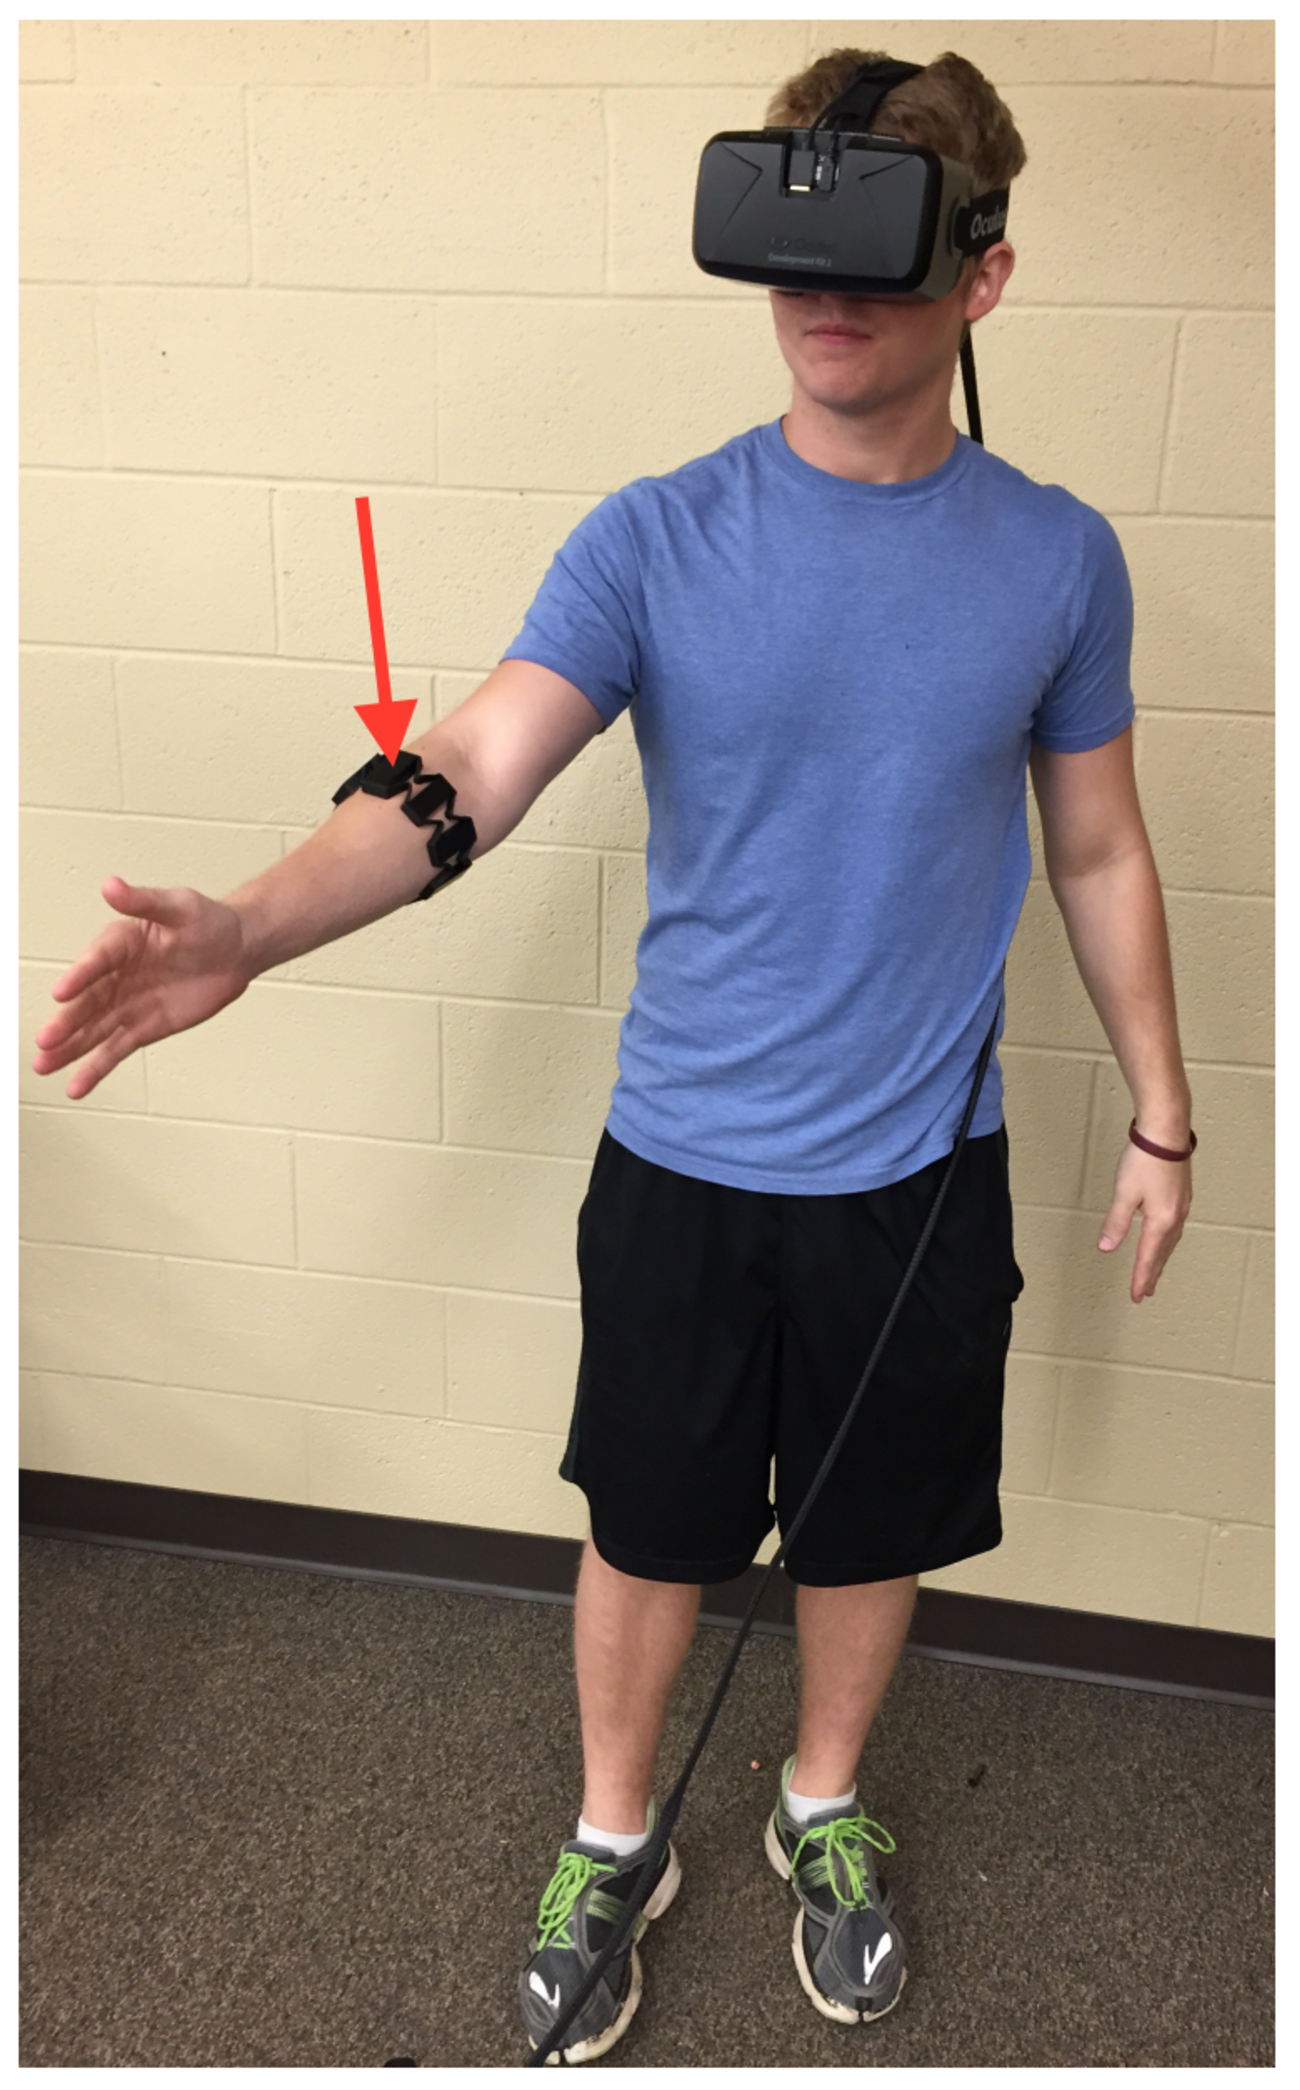
\includegraphics[scale=.25]{morgan_and_myo.eps}
  \caption{User wearing a Myo armband}
  \label{fig:morgan}
\end{figure}
The Myo armband is a wearable band (seen in Figure \ref{fig:morgan}).
To use our arm swinging method, subjects wore the Myo armband on the thickest part of their forearm, just below their elbow.
The armband was adjusted so that it was comfortably snug, not sliding on the users' arms when they moved.
To use the walking in place method, subjects wore the Myo armband about midway on their calves.
The exact position varied between users, but again, we adjusted it to be comfortably snug.
The armband fits sizes between 7.5in and 13in in circumference
by adding or removing the expanders that come with the product.

The Myo armband has two types of sensors:
medical grade stainless EMG sensors
and a nine axis inertial internal measurement unit (IMU).
The IMU contains a three-axis gyroscope, a three-axis accelerometer, and a three-axis magnetometer.
Thus, the Myo SDK provides several kinds of spatial data:
orientation in terms of pitch, yaw and roll;
acceleration vector data which represents the acceleration of the armband;
and angular velocity data provided by the gyroscope.
It is important to note that the IMU in the Myo armband can accurately measure the orientation of the arm (roll, pitch, yaw);
position data is obtained from these angles.
It can achieve a sampling rate of 50 Hz.
All data from the Myo is communicated via Bluetooth to a computer.
Participants wore the armband
with the Myo logo facing directly up when their arms were
at their side as seen in Figure \ref{fig:morgan}.
As a result, the orientation sensor on the device is oriented to everyone’s arm in a similar way.





\subsubsection{Myo arm swinging}
We wanted to test the locomotion method of our previous work \cite{previousMYO}
to walking in place and physical locomotion.
We note that we only used one armband in this locomotion method.
Unlike our previous work \cite{previousMYO},
users were not forced to move with both arms.
They could navigate however was most comfortable for them,
and for several users, this meant just moving one arm.

This is possibly a shortcoming,
but could be easily fixed by requiring participants to move both of their arms,
even though only one arm is relaying information.
This approximation works well because when one arm is swinging, the other arm usually swings too.

To infer steps from arm movement,
we basically calculated the velocity in the $y$-direction.
We note that when one swings their arms,
the movement is mostly in the $z$ and $y$ positions.
We chose to measure the $y$-velocity because it was consistent regardless which way the user was facing.
Additionally, this helps prevent accidental movement due to gesticulation.
If the user moved their arms too much in the $x$ or $z$ direction,
we counted it as gesticulation and would not move the user forward.
Later, we discuss possible alternatives to this algorithm.

To stop moving, participants stopped moving their arms.
With this arm swinging algorithm, if subjects swung their arms faster,
they would propel themselves forward faster due to the increased velocity.

\subsubsection{Myo marching}
As we have previously had success with WIP \cite{Williams:2011:EWP},
we tried to use the reliable and precise Myo base to create an inexpensive WIP system.
% Our novel approach presented in this work allows the user to walk in place with Myo.
% easier to implement;
This system was easier to implement.
Using two Kinects required that we set up a virtual private network to send skeletal data from both Kinects
to the computer running the environment.
Myo armbands use Bluetooth.
We obtained the data from both armbands on one computer,
and Unity supported using two out of the box.
As the EMG sensors of the Myo armbands are designed for the user's arm,
the EMG data gathered from the leg was useless and disregarded.

We instead relied on the accelerometer data.
We simply measured the change in velocity from the Myo armband.
Users were able to walk in a way that is most comfortable to them rather than march.
We suggested that the users moved mostly by raising their calves up and down.
Like the arm swing method, we measure change in the $y$-position.
However, since the knee has fewer degrees of movement,
we do not need to account for gesticulation.
We also made the assumption that one leg is stationary while another is moving.
This is not accurate for actual walking, but works well enough for walking in place.
Thus, we simply summed the change in differences for each leg.
Later, we discuss improvements and alternatives to this algorithm.
% look at change in gyroscope in y to see if rotating...

%more robust, more precise
The Myo armband avoids the problem of occlusion faced by the Kinect.
No optical data is needed as data is read directly from the skin of the user.
Additionally, as we used the data from the accelerometer,
users had more precise control over their movement.
The faster they walked in place, the faster they moved in the VE.
They could quickly stop and move slightly and comfortably.

\subsection{Physical Tracking}
In order to compare our two algorithms of walking in place and arm swinging to the gold standard of tracked locomotion,
we had to implement tracked locomotion.
Users would physically rotate and move,
and their rotation and position in the virtual environment would be similarly updated.
Unfortunately, implementing this was unnecessarily complicated.
Even though we easily obtained tracking data through VRPN in Vizard,
we could not replicate this process in Unity.
We tried various approaches and many configurations to obtain tracking data in Unity,
but none of them worked.
Finally, we settled on using inter-process communication.
Again, we tried many things,
but finally settled on Vizard outputting the tracking information to a file,
then Unity reading this file, thus getting the tracking information.

\newpage
\section{Experiment}
We compared arm swinging to Myo walking in place to physical walking
in order to find whether either of these locomotion methods could replace physical walking
in consumer virtual environment systems.
We tested 12 subjects on their spatial orientation and perception of distances in the environment
using within-subjects design.
After a user finished all three navigation methods,
we asked them a series of questions.

\subsection{Spatial Orientation}
As we have done before \cite{Wilson:2014,Williams:2011:EWP},
we conducted spatial orientation tasks for each navigation method.
For each condition, the user would memorize the positions of 6 objects
placed around the environment on columns (Figure \ref{fig:objects}).
The heights of the cylinders varied so that the top of the objects were always at the same level.
After the user had memorized the locations of the objects,
the tests would begin.

There were six testing locations;
they were the same between navigation methods as well as between subjects.
For each subject and for each navigation method, we randomized the order in which
the user would visit the testing sites to account for effects of order on the results.
At each location, the user would turn to face three different objects.
The order of these three objects was randomized between locations, navigation methods, and subjects.

A testing location and a testing orientation marker
(pictured in Figure \ref{fig:objects} as the red cylinder and the green sphere, respectively)
showed the user from where we would test them.
When the user was close enough,
the cylinder would turn green.
At this point, the user's position would freeze and the objects would disappear.
Then, they would turn to face the sphere until it turned green.
Thus, all participants were tested at the same location and orientation,
meaning that the correct angles of response were the same between subjects.

\begin{figure}[h]
  \centering
  \includegraphics[scale=.25]{objects.png}
  \caption{An example view of the environment}
  \label{fig:objects}
\end{figure}

After the third object, the user was told to turn back to face the sphere
so that they did not receive any feedback.
For each object, we recorded the latency of the subject, or how long they took to turn to face it,
the correct angle of response,
and their turning error.
Latency was measured from the time the object was identified
until subjects said that they had completed their turning movement and were facing the target.
Turning errors were measured as the difference between the direction the user was facing
and the correct angle of response.
There were six testing locations for each locomotion condition, and three objects to turn to face at each location.
Thus, the user turned to face objects 18 times per condition.

\subsection{Distance Perception}
We additionally tested users on their distance perception in the virtual environment.
% citation needed
Users consistently underestimate distances in virtual environments
\cite{Plumert:2005:DPR:1077399.1077402,Renner:2013:PED:2543581.2543590},
and we wanted to see whether our locomotion methods would remedy or maintain this.

After a user was finished with their spatial orientation tasks,
we removed the objects and set them in the middle of the room if they were in the tracking condition.
An avatar would appear either 10, 20, 30, or 40 Unity units away from the user,
where about 8 Unity units was 1 meter for us.
After the user saw where the avatar was, the display would go black,
and the user would navigate to where they thought the avatar was.
We tested each distance twice.
The order of the distances was randomized between navigation methods and between subjects.

We recorded
the correct distance,
how far the user was from the avatar when they said they were at the avatar,
and how long it took the user to move to that position.

\subsection{Survey Questions}
We asked users the following questions:
\begin{itemize}
\item What was your favorite locomotion method?
\item Describe any problems with any of the locomotion methods.
\item Did you have any strategies?
\item On a scale from 1-5, 5 being the most comfortable/natural,
  how comfortable/natural was each locomotion method?
\item Did you feel nauseous at any point?
\item Did the movement seem realistic? (specify for each locomotion method)
\end{itemize}

\newpage
% maybe make these results side by side?
\section{Results}
To determine the relative performance between the three conditions,
we assessed turning error, turning latency,
distance perception, and user feedback.
The mean and median turning errors follow.

\begin{figure}[h]
  \centering
  \begin{minipage}[h]{.45\linewidth}
    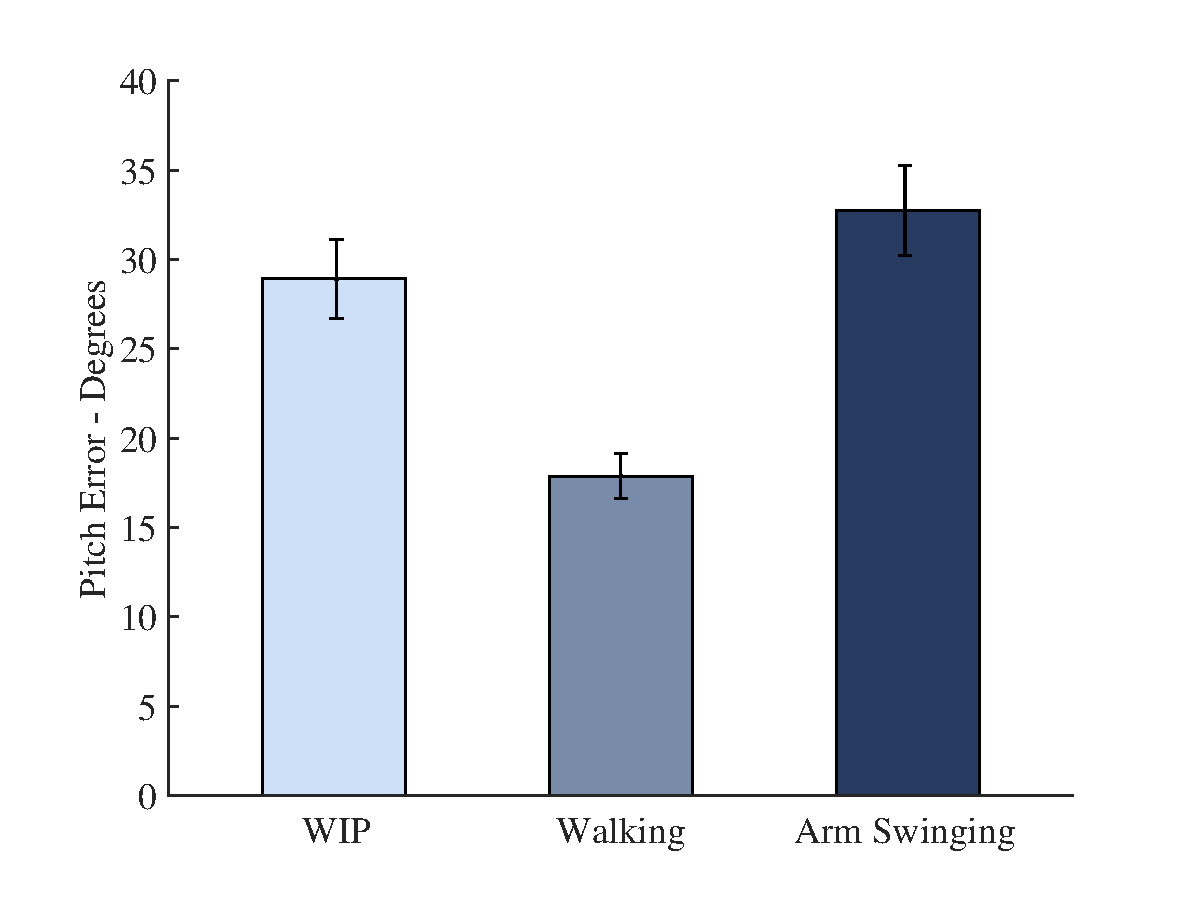
\includegraphics[scale=.4]{te_mean.eps}
  \end{minipage}
  \quad
  \begin{minipage}[h]{.45\linewidth}
    \includegraphics[scale=.4]{te_median.eps}
  \end{minipage}
  \caption{Mean and Median Turning Errors}
  \label{fig:turning_errors}
\end{figure}

This large difference between the two shows that
there were a couple of users whose performance was exceptionally poor.

Analyzing our data,
we found a significant effect of condition on turning error:
F(2, 10) = 6.533 and p = 0.015.
T-tests further revealed a significant difference between the walking in place condition
and the physical tracking condition
and between the arm swinging condition and the walking condition.
One can can see this in the level of difference of turning errors in Figure \ref{fig:turning_errors}.

One can see below that users responded in a consistent amount of time for each condition.
We measured the latency to see whether a user was lost in the environment.
We hypothesized that if they were, then they would take longer to respond as to where an object was.

\begin{figure}[h]
  \centering
  \begin{minipage}[h]{.45\linewidth}
    \includegraphics[scale=.32]{figures/lat_mean.eps}
  \end{minipage}
  \quad
  \begin{minipage}[h]{.45\linewidth}
    \includegraphics[scale=.32]{figures/lat_median.eps}
  \end{minipage}
  \caption{Mean and Median Turning Latencies}
  \label{fig:turning_latencies}
\end{figure}

\clearpage
The results for blind walking follow in Figure \ref{fig:blind-walking-latencies}.
\ref{fig:blind-walking-differences} and \ref{fig:blind-walking-latencies}.
\begin{figure}[h]
  \centering
  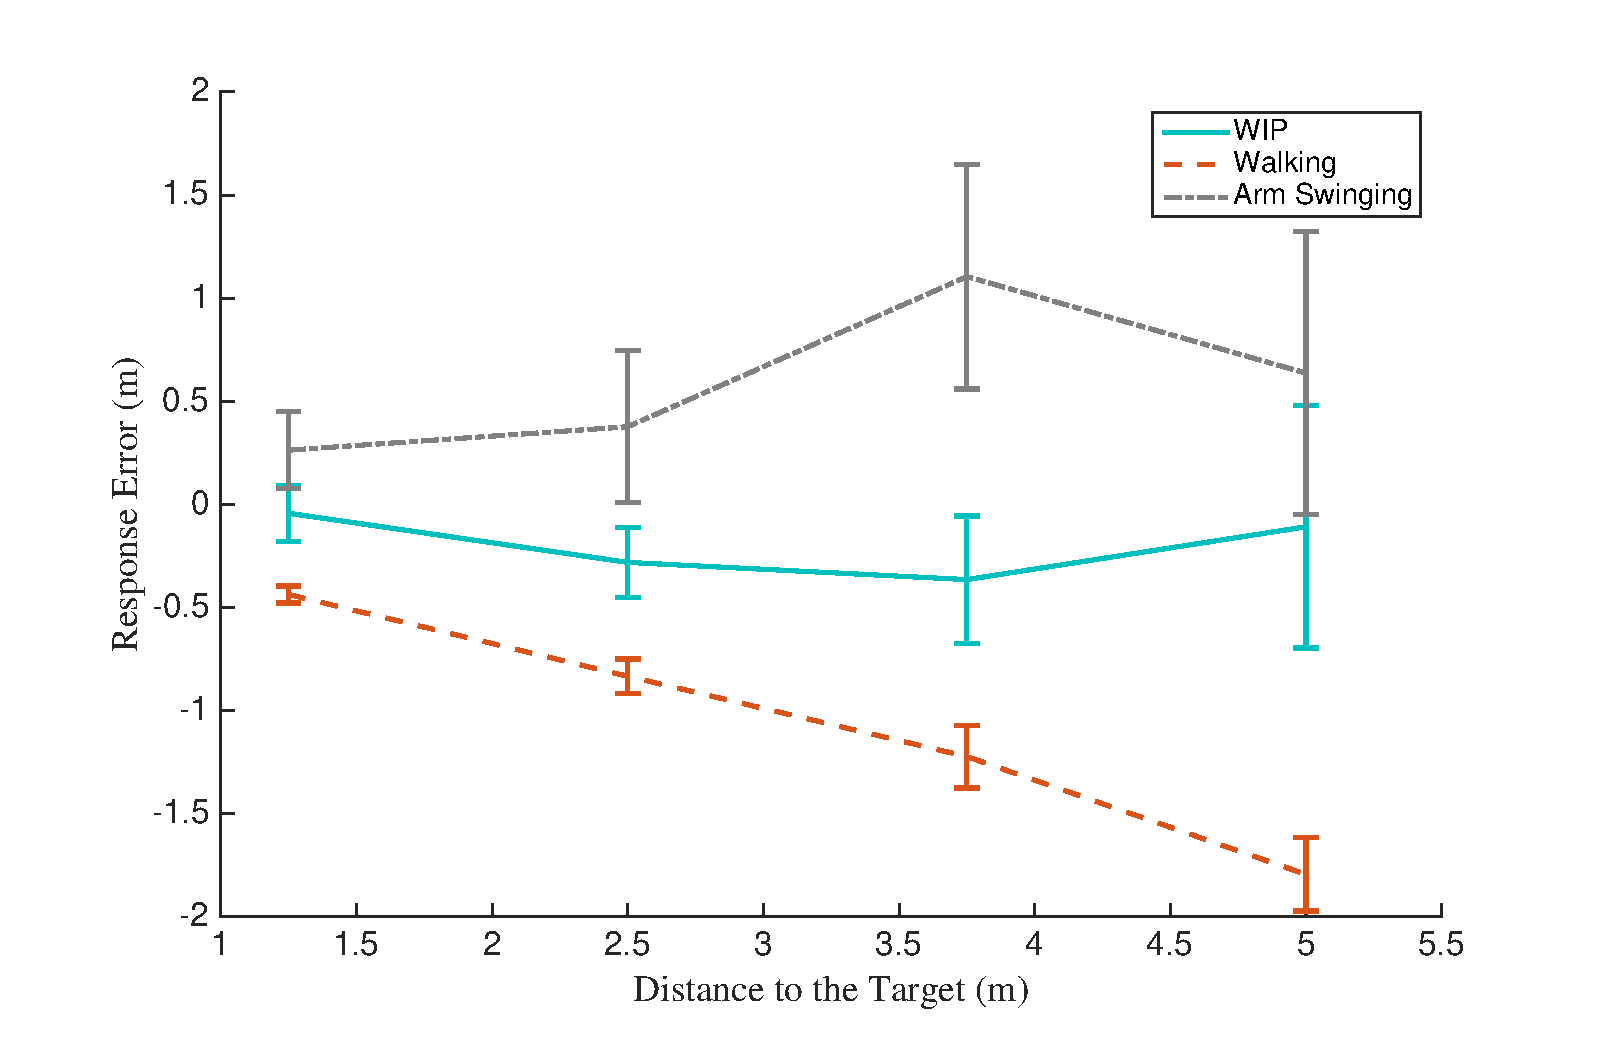
\includegraphics[scale=.35]{figures/blind_walking.eps}
  \caption{Blind Walking Differences}
  \label{fig:blind-walking-differences}
\end{figure}
\begin{figure}[h]
  \centering
  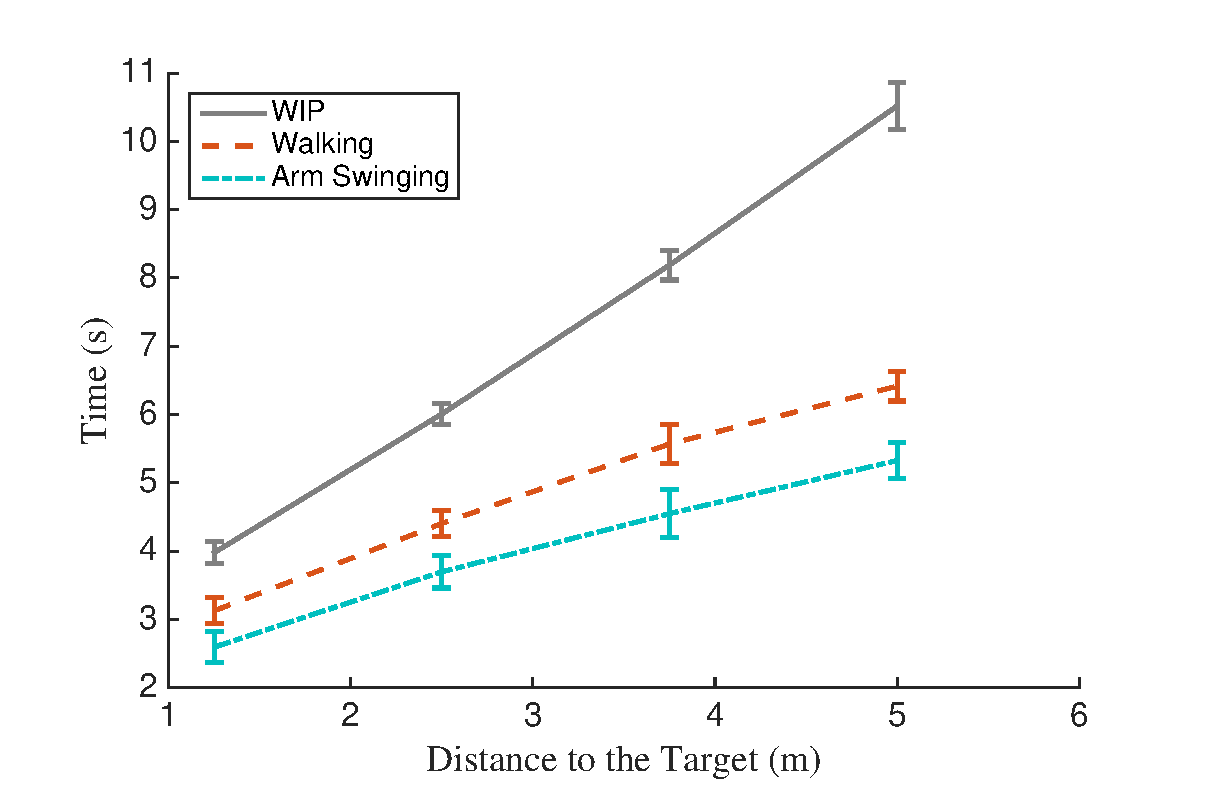
\includegraphics[scale=.45]{figures/blind_walking_latency.eps}
  \caption{Blind Walking Latencies}
  \label{fig:blind-walking-latencies}
\end{figure}

We tested distance perception to see whether users underestimated distances as
other studies have shown. %citation needed
It is interesting to see that users over-walked or overestimated distances in the arm swinging condition.
It is also interesting to see that people performed reasonably well with walking in place,
but they took longer to respond.
What these results might demonstrate instead is that users were not well-adjusted to the locomotion methods.
It might be that rather than successfully estimating the distances
in the walking in place condition,
they did not know how far they were moving and accidentally moved closer to the correct location.
Thus, similarly for arm swinging, users did not overestimate the distance,
but instead underestimated how far one swing would take them in the virtual environment.
% could be that people underestimated distances in wip,
% but without feedback walked farther than they would otherwise

\clearpage
\section{User Feedback}
The results from the questions we asked each of the twelve users follow.
The average ratings of the comfort/how natural each locomotion method felt were
3 out of 5 for walking in place,
4.5 out of 5 for physical walking,
and 2.7 for arm swing.
People clearly preferred physical walking--
all but four of the twelve participants listed it as their favorite.
Interestingly, users might have thought that another method was their favorite,
but they thought that physical locomotion was more natural.

Two users reported being nauseous.

\begin{itemize}
\item One user exclaimed ``very cool'' in the arm swinging condition.

\item Two users held their arm in a prone position,
  and moved it up and down to move forward in the arm swinging condition.
  This was interesting because two users found this approach,
  which was not similar to how they actually walk.

\item Users reported that the walking in place and arm swinging seemed a little ``un-smooth.''
  A user thought that walking in place was most realistic besides actual walking.

\item Another user said that the walking in place was kind of weird--
  they felt they would go an inconsistent distance with each step.
  ``The arm swing wasn't bad.''

\item Another user said that arm swinging did not seem as realistic.

\item A user said that walking in place was not realistic.
  This user said ``this is unnerving'' on arm swinging.
  They also felt that the two Myo locomotion methods moved them forward in smaller increments than real walking.

\item A user said that it was hard to tell how far they moved in the walking in place condition.

\item A user preferred arm swinging over walking in place.

\item Another user said that arm swinging did not feel like their full stride length.

\item A user said that the arm swinging was the hardest and that they did not get used to it.
  They said ``this is so hard,'' during that condition,
  then reported the above statement when we asked the above questions.

\item Another user said that arm swinging was fast, or that they did not get used to it.

\item Yet another user said that though the arm swinging was the least natural,
  they liked it because they could move around the quickest in it.
\end{itemize}

It was interesting to see users take really small steps in the walking in place condition.
Some users started out swinging both arms then switched to moving a single arm.

These inconsistent opinions might have been remedied by making sure that each
user used the locomotion methods similarly.
As we had it, they were free to experiment and find what was most natural for them.
This probably led to the wide array of opinions on the different locomotion methods.

\newpage
\section{Discussion}
% talk about maybe since we didn't enforce people to use both arms...
To briefly summarize our results,
we found that physical locomotion outperformed our Myo algorithms in terms of turning error,
we did not find a significant difference between performance of our two Myo algorithms in terms of turning error,
and users were strangely accurate at walking to the correct distance in the walking in place condition.
But as mentioned above, this might point to an underestimation of how far the user was moving
now that they did not have visual feedback rather than an accurate perception of distances.

Our previous experiment \cite{previousMYO} with the Myo armband shows that although the
proprioceptive cues of the arm swinging method do not exactly match physical walking,
the cyclic repetition of movement is similar to walking
as humans swing their arms when they walk.
Moreover, Zehr et al. \cite{zehr} point out that both the arms and legs are coordinated by central pattern generators (CPG),
which are biological neural networks that produce rhythmic patterned outputs without sensory feedback.
Thus, arm and leg movements are regulated
by CPG activity and sensory feedback.
They also explain that the
strength of coupling between the legs is stronger than that between the arms.
We hypothesize that the arm and leg movements prime the sensory motor system to process optical flow.
This idea of the movement condition priming the sensory motor system is consistent with the literature
\cite{Engel:2008VRST,Nitzsche2004:Presence,Razzaque2001:Eurographics,Steinicke:2010,Williams2006:APGV}.

Additionally, researchers \cite{Engel:2008VRST,Nitzsche2004:Presence,Razzaque2001:Eurographics,Steinicke:2010}
have previously designed an algorithm
that imperceptibly rotates the virtual environment so that the physical locomotion of the user fits within the
confines of the tracking system.
Again, researchers are able to successfully manipulate the mapping between normal physical walking
and visual flow in such a way that spatial orientation is maintained.
This provides the user with an opportunity to explore a virtual space
larger than the tracking space.
This is an alternate approach to the one we have taken,
but it still works towards providing spatial orientation in virtual environments
while avoiding the spatial constraint of virtual environments fitting within the physical location.

%%SCIENCE ABOVE

We believe that our new Myo navigation methods, just as our previous locomotion methods,
will be superior to joystick locomotion because
users have difficulty mapping optical flow to pushing forward on a joystick.
In line with our prior WIP research,
our current work and arm swinging studies suggest that physical motion and cyclic action add
value to users' spatial updates.
But rather than focusing on beating the lowest common method,
we sought to emulate or outperform the current gold standard: physical locomotion.
Thus, we directly compared our methods to physical locomotion rather than the joystick.

Due to the fact that we were not able to show a statistical significant difference between
walking in place and arm swinging
and the fact that users had conflicting opinions on which of the two Myo methods was better,
we hypothesize that either method could be a viable way to explore a large virtual environment.
The armband is easy to operate and our algorithms are simple and robust.
Methods of navigation based on the Myo armband do not suffer from either space limitations or occlusion.

Our users gave us an idea for another condition:
physically walking with the Myos around their calves.
Especially when switching from physical locomotion to walking in place,
the users would take some initial steps before we reminded them to walk \emph{in place}.
We noticed that their movement in the virtual environment closely mimicked
how they were physically moving.
This still requires a large amount of space like a tracking system,
but is orders of magnitude cheaper.
Ways of improving our walking in place algorithm would lend themselves naturally to this new condition.


We could also improve the arm swinging and walking in place algorithms to more closely mimic walking.
Change in velocity seems to work fine for now,
but it is simple.
It is worth exploring whether we can have fewer false positives due to gesticulation or turning.
One initial idea to check if a user is turning is to see whether
their rotation in the $y$-direction is greater than some value.
This could be done either with the gyroscope on the Myos,
or by checking the angular velocity of the Oculus.
One idea is to train a neural net to identify steps of the user.
Another is to aggregate more sensor data from the Myos into whether a movement is a step or not.

Finally, another idea which we are considering is using participants' phones as movement sensors.
Like the Myo bands, most smart phones are equipped with an accelerometer and gyroscope;
this would avoid the cost of buying and using additional equipment.
We would need to consider the number of different phones
and come up with a way of getting the information we need regardless of the phone.

All of this work is for the goal of making virtual environments an accessible part of everyday life.
We continue to try to test these inexpensive methods to make systems more accessible to consumers,
in terms of both expense and space.
% 9 tables, illustrations, figures
% 10 appendices
% 11 glossary
% 12 list of symbols and or abbreviations
% 13 bibliography
\newpage
\addtotoc{References}
\bibliographystyle{amsalpha}
\bibliography{bib}
\nocite{*}
\end {document}

%  LocalWords:  isomorphy subsequences bijection embeddings Myo Myos
%  LocalWords:  proprioceptive electromyography Advisor WIP Kinect
%  LocalWords:  USD LocalWords
